%%%%%%%%%%%%%%%%%%%%%%%%%%%%%%%%%%%%%%%%%
% Short Sectioned Assignment LaTeX Template Version 1.0 (5/5/12)
% This template has been downloaded from: http://www.LaTeXTemplates.com
% Original author:  Frits Wenneker (http://www.howtotex.com)
% License: CC BY-NC-SA 3.0 (http://creativecommons.org/licenses/by-nc-sa/3.0/)
%%%%%%%%%%%%%%%%%%%%%%%%%%%%%%%%%%%%%%%%%

% \documentclass[paper=a4, fontsize=11pt]{scrartcl} % A4 paper and 11pt font size
\documentclass[11pt, a4paper]{book}
\usepackage[T1]{fontenc} % Use 8-bit encoding that has 256 glyphs
\usepackage[utf8]{inputenc}
\usepackage{fourier} % Use the Adobe Utopia font for the document - comment this line to return to the LaTeX default
\usepackage{listings} % para insertar código con formato similar al editor
\usepackage[spanish, es-tabla]{babel} % Selecciona el español para palabras introducidas automáticamente, p.ej. "septiembre" en la fecha y especifica que se use la palabra Tabla en vez de Cuadro
\usepackage{url} % ,href} %para incluir URLs e hipervínculos dentro del texto (aunque hay que instalar href)
\usepackage{graphics,graphicx, float} %para incluir imágenes y colocarlas
\usepackage[gen]{eurosym} %para incluir el símbolo del euro
\usepackage{cite} %para incluir citas del archivo <nombre>.bib
\usepackage{enumerate}
\usepackage{hyperref}
\usepackage{graphicx}
\usepackage{tabularx}
\usepackage{booktabs}

%
% Para insertar código
%

\usepackage{listings}
\usepackage{color}
\definecolor{lightgray}{rgb}{.9,.9,.9}
\definecolor{darkgray}{rgb}{.4,.4,.4}
\definecolor{purple}{rgb}{0.65, 0.12, 0.82}

\lstdefinelanguage{JavaScript}{
  keywords={typeof, let, const, new, true, false, catch, function, return, null, catch, switch, var, if, in, while, do, else, case, break},
  keywordstyle=\color{blue}\bfseries,
  ndkeywords={class, export, boolean, throw, implements, import, this},
  ndkeywordstyle=\color{darkgray}\bfseries,
  identifierstyle=\color{black},
  sensitive=false,
  comment=[l]{//},
  morecomment=[s]{/*}{*/},
  commentstyle=\color{purple}\ttfamily,
  stringstyle=\color{red}\ttfamily,
  morestring=[b]',
  morestring=[b]"
}

\lstset{
   language=JavaScript,
   backgroundcolor=\color{lightgray},
   extendedchars=true,
   basicstyle=\footnotesize\ttfamily,
   showstringspaces=false,
   showspaces=false,
   numbers=left,
   numberstyle=\footnotesize,
   numbersep=9pt,
   tabsize=2,
   breaklines=true,
   showtabs=false,
   captionpos=b
}

%%%%%%%%%%%%%%%%%%%%%%%%%%%%%%%%%%%%

%problema fuentes tamaños
\usepackage{lmodern}

\usepackage[table,xcdraw]{xcolor}
\hypersetup{
	colorlinks=true,	% false: boxed links; true: colored links
	linkcolor=black,	% color of internal links
	urlcolor=cyan		% color of external links
}
\renewcommand{\familydefault}{\sfdefault}
\usepackage{fancyhdr} % Custom headers and footers
\pagestyle{fancyplain} % Makes all pages in the document conform to the custom headers and footers
\fancyhead[L]{} % Empty left header
\fancyhead[C]{} % Empty center header
\fancyhead[R]{Víctor González Argudo} % My name
\fancyfoot[L]{} % Empty left footer
\fancyfoot[C]{} % Empty center footer
\fancyfoot[R]{\thepage} % Page numbering for right footer
%\renewcommand{\headrulewidth}{0pt} % Remove header underlines
\renewcommand{\footrulewidth}{0pt} % Remove footer underlines
\setlength{\headheight}{13.6pt} % Customize the height of the header

\usepackage{titlesec, blindtext, color}
\definecolor{gray75}{gray}{0.75}
\newcommand{\hsp}{\hspace{20pt}}
\titleformat{\chapter}[hang]{\Huge\bfseries}{\thechapter\hsp\textcolor{gray75}{|}\hsp}{0pt}{\Huge\bfseries}
\setcounter{secnumdepth}{4}
\usepackage[Lenny]{fncychap}


\begin{document}

	% Plantilla portada UGR
	\input{portada/portada}

	% Plantilla prefacio UGR
	\thispagestyle{empty}

\begin{center}
{\large\bfseries MemeHub \\ Edición Online de Imágenes }\\
\end{center}
\begin{center}
Víctor González Argudo\\
\end{center}

%\vspace{0.7cm}

\vspace{0.5cm}
\noindent{\textbf{Palabras clave}: \textit{Javascript, React.js, Editor de Imágenes, Memes, Software Libre}}
\vspace{0.7cm}

\noindent{\textbf{Resumen}\\}
	En la actualidad los editores de imágenes online, concretamente los especializados en
	edición de memes, 

\cleardoublepage

\begin{center}
	{\large\bfseries MemeHub \\ Online Image Editing}\\
\end{center}
\begin{center}
	Víctor González Argudo\\
\end{center}
\vspace{0.5cm}
\noindent{\textbf{Keywords}: \textit{Javascript, React.js, Image Editor, Memes, Open Source}}
\vspace{0.7cm}

\noindent{\textbf{Abstract}\\}
	Currently the online image editors, being more specific the online meme generators, are
	not as good as they could be. 


\cleardoublepage

\thispagestyle{empty}

\noindent\rule[-1ex]{\textwidth}{2pt}\\[4.5ex]

D. \textbf{Juan Julián Merelo Guervós}, Profesor(a) del departamento de Arquitectura y Tecnología de 
Computadores de la Universidad de Granada.

\vspace{0.5cm}

\textbf{Informo:}

\vspace{0.5cm}

Que el presente trabajo, titulado \textit{\textbf{MemeHub}},
ha sido realizado bajo mi supervisión por \textbf{Víctor González Argudo}, y autorizo la defensa de dicho trabajo ante el tribunal
que corresponda.

\vspace{0.5cm}

Y para que conste, expiden y firman el presente informe en Granada a Junio de 2018.

\vspace{1cm}

\textbf{El/la director(a)/es: }

\vspace{5cm}

\noindent \textbf{Juan Julián Merelo Guervós}

\chapter*{Agradecimientos}

En primer lugar, me gustaría agradecer a mi tutor, JJ, tanto por el apoyo durante la realización
de este proyecto, como por su ayuda en otros ámbitos relacionados con el mundo de la informática.
\\\\




	% Índice de contenidos
	\newpage
	\tableofcontents

	% Índice de imágenes y tablas
	\newpage
	\listoffigures

	% Índice de código
	\newpage
	\renewcommand\lstlistingname{Código}
	\renewcommand\lstlistlistingname{Índice de código}
	\lstlistoflistings

	% Si hay suficientes se incluirá dicho índice
	%\listoftables 
	%\newpage

	% Introducción 
	\chapter{Introducción}

%Por qué hay necesidad de mi apliación 

%los memes se hacen con imagenees en linea noirmalmente

%importancia de compartir imagenes facilmente en las

Este proyecto es software libre, y está liberado con la licencia \cite{gplv3}.
\\\\
Actualmente, 

	% Descripción del problema y hasta donde se llega
	%\chapter{Descripción del problema}

Este proyecto pretende facilitar en la medida de lo posible la edición de imágenes que requieren
de una edición rápida y ligera, como es principalmente el caso de los memes.
\\\\
Actualmente, la mayoría de usuarios utilizan aplicaciones locales, instaladas en el propio
ordenador, grandes y pesadas para la edición de imágenes que requieren de cambios simples, 
como puede ser: añadir texto, superponer imágenes encima de una base o crear formar geométricas
para resaltar alguna parte de la imagen base.
\\\\
Los programas de edición locales, como Photoshop o MSPaint, son pesados, con largos tiempos de
carga y lo peor, requieren descargar tanto las fuentes como almacenar el resultado de forma local.
\\\\
El objetivo de este proyecto es dar una solución mejor a este problema, siguiendo la tendencia
actual del desarrollo en la actualidad, que son las aplicaciones web (SaaS, Software as a Service), 
evitando tener que efectuar ninguna descarga y dando la posibilidad de cargar, editar y exportar sin 
necesidad de emplear el almacenamiento local.




	% Estado del arte
	% 	1. Crítica al estado del arte
	% 	2. Propuesta
	\chapter{Estado del arte}

La motivación de este proyecto surge precisamente por el estado actual de los editores de imágenes. 
La mayoría de usuarios, edita el contenido que sube online desde una aplicación local instalada en 
su ordenador (Microsoft Paint, Photoshop), o en el caso de los que emplean aplicaciones en la nube, 
descargan sus imágenes para luego resubirlas a sus redes.
Concretamente los memes suelen ser ediciones especialmente simples, donde se añade un texto, 
se superponen varias imágenes o se dibuja algo encima de una imagen base.
\\\\
Este proyecto tiene como objetivo tratar este problema y evitar en la medida de lo posible el uso 
del almacenamiento local de imágenes, tanto para crear, como para subir el contenido ya editado. 
\\\\
Además, existen editores especialmente dedicados a los memes que te aportan varias plantillas
base, pero tienen muchas desventajas, en primer lugar los mas populares son toscos y desfasados,
con interfaces poco interactivas y sin mucha personalización, la edición es lenta y están faltos
de herramientas esenciales en el diseño de memes actual. 
\\\\
Desde hace años los memes han 
evolucionado y ya no se basan en una simple imagen con un texto, suelen ser una superposición
de varias imágenes, con elementos resaltados, muchos textos pequeños con diferentes estilos
y filtros o efectos.

\begin{figure}[!h]
\centering
    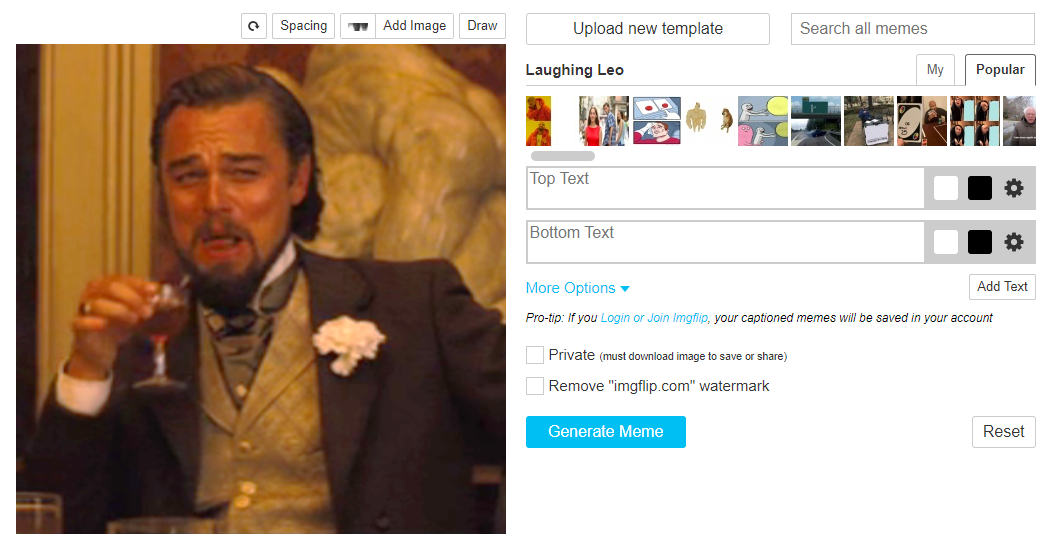
\includegraphics[scale=0.4]{img/imgflip.png}
\caption{imgflip, editor de memes popular.}
\end{figure}
	
	% Análisis del problema
	% 1. Análisis de requisitos
	% 2. Análisis de las soluciones
	% 3. Solución propuesta
	% 4. Análisis de seguridad
	\chapter{Análisis del problema}

Como hemos comentado en el anterior capítulo, la principal competencia actual está 
bastante anticuada, especialmente en el ámbito de los memes.
\\\\
Para convertir este proyecto en algo viable y competitivo, deberemos asegurarnos de que
el usuario tenga una experiencia fluída, en contraposición con el resto de editores.
\\\\
Una de las principales carácterísticas que debe tener es poder cargar, editar y subir sin
necesidad de descargar nada en ningún momento.
\\\\
El editor debe ser simple y rápido, cargar rápido, responder rápido
y, en general, resaltar en la medida de lo posible en todos los aspectos 
que fallan en los editores locales convencionales.
\\\\
Además otro de los objetivos del proyecto es la posibilidad de llevar a 
cabo todo esto manteniendo al servidor libre de carga, ya que, los cálculos
y las ediciones sobre contenido multimedia consume bastante capacidad de 
procesamiento y de red ya que tendríamos que enviar el multimedia al servidor.
\\\\
Lo mas lógico por ende para solucionar esto es hacer que la aplicación sea 
puro front-end, es decir, emplear un esquema donde el servidor se desentiende
tras enviar el software que se ejecute en el navegador.
\\\\
Para este tipo de aplicaciones está bastante generalizado el uso de frameworks 
y bibliotecas front-end como Vue.js o React.js.
\\
Tras investigar y comparar las diferentes posibilidades finalmente nos decantamos
por el uso de React.js ya que era el framework que mejor permitía dar
la experiencia de usuario que deseamos, una aplicación reactiva, donde tenemos
un gran control sobre el rendimiento durante el desarrollo gracias al 
desarrollo enfocado a componentes de React.js que nos permitirá actualizar
en cada momento sólo algunas partes de la aplicación.  
\\\\
Tras la elección de la biblioteca que vamos a utilizar.
hemos planteado que el editor esté formado por las siguientes partes:

\begin{figure}[!h]
    \centering
    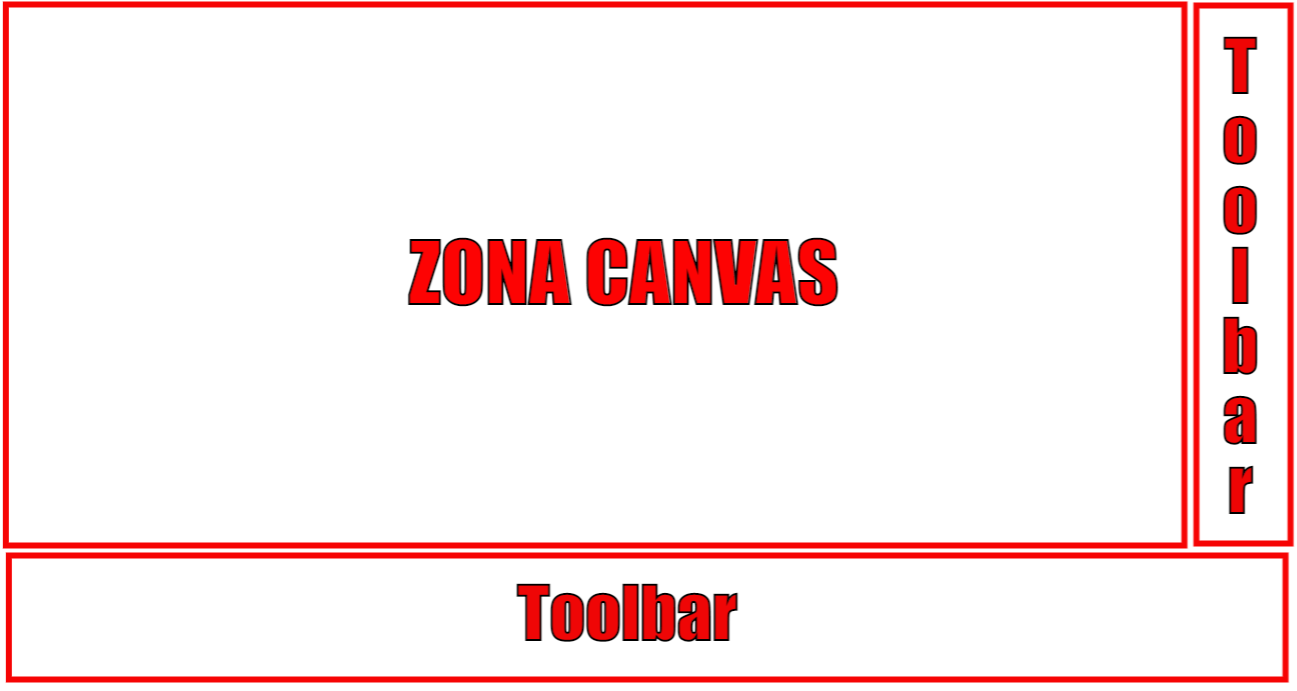
\includegraphics[scale=0.30]{img/ESQUEMA_ABSTRACTO.png}
    \caption{Esquema de las partes que debería tener el editor}
\end{figure}

Como vemos es una estructura simple, con partes claras y diferenciadas, 
que tiene en cuenta todos los objetivos planteados anteriormente.

	\chapter{Planificación}

\section{Metodología utilizada}
    Para la realización de este proyecto se ha seguido una metodología ágil o 'Agile', esta metodología
    es especialmente buena para los proyetos que necesitan de mucha flexibilidad, por ende, por 
    la naturaleza de algo como una aplicación de edición de imagen, que es algo que invita fácilmente a 
    añadir nuevas funcionalidades y a cambiar o adaptar antiguas al nuevo contenido que se añada,
    ha sido escogida para el desarrollo de este trabajo.
    \\\\
    Se ha escogido Kanban como metodología ágil para el desarrollo de este proyecto.
    Como marca el desarrollo ágil, se parte de la idea que queremos implementar, un editor
    con las partes y funcionalidades que hemos definido en anteriores capítulos. Y se comienza
    a descomponer en problemas mas pequeños, que a su vez se descomponen en problemas aún mas 
    pequeños hasta llegar a funcionalidades básicas. 
    Estas funcionalidades básicas son las llamadas historias de usuario (HUs) que se redactan 
    desde el punto de vista del usuario que vaya a utilizar esa funcionalidad básica.

    \begin{figure}[!h]
      \centering
      \noindent\makebox[\textwidth]{
        
\includegraphics[scale=0.9]{img/ejemplohu.png}}
      \caption{Ejemplo de una historia de usuario empleada en el proyecto}
    \end{figure}
    

%- Busqué librerias y cosas mientras seguí aprendiendo React (planificacion)

%- Despues de unos cuantos proyectos de prueba y elegidas las librerias me lancé con el editor
        %La implementación del software se ha dividido en hitos. Estos, han sido definidos en Github
    %y cada uno de ellos contiene un grupo de \textit{issues} que se corresponden con las distintas
    %mejoras que se han ido incorporando al software a lo largo de su desarrollo.


\newpage
\section{Seguimiento del desarrollo}
Para el seguimiento y gestión del desarrollo se ha utilizado el software de control de versiones
git\cite{git} en la plataforma Github\cite{Github}.
\\
Se ha creado un github project y se ha utilizado una tabla Kanban para gestionar las historias 
de usuario y las issues del proyecto.
\\\\
El Kanban del proyecto puede verse en el siguiente enlace:
\url{https://github.com/bytevictor/memeHub/projects/1}

\begin{figure}[!h]
  \centering
  \noindent\makebox[\textwidth]{
    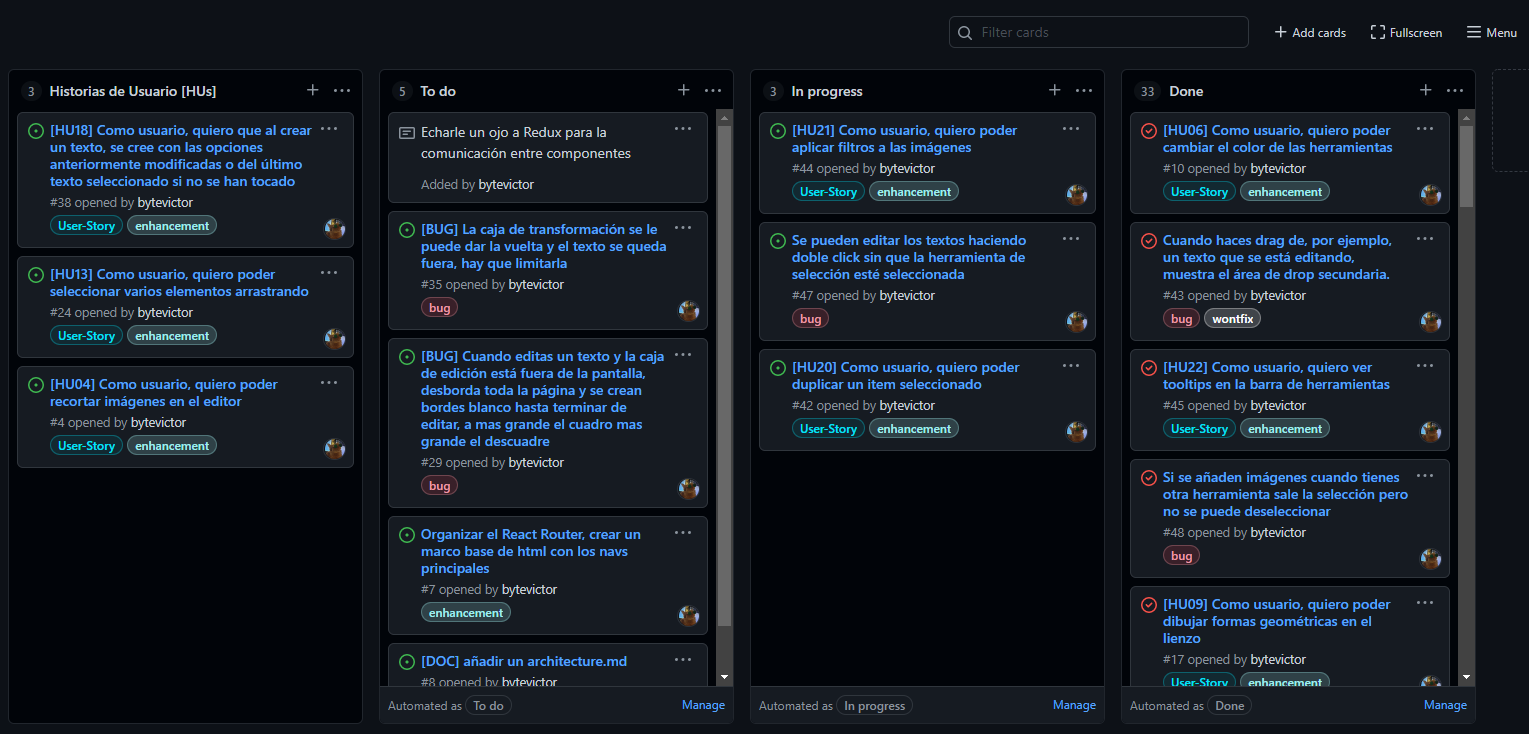
\includegraphics[scale=0.4]{img/kanban.png}}
  \caption{Tabla Kanban del proyecto de Github de MemeHub.}
\end{figure}

	% Desarrollo bajo sprints: 
	% 	1. Permitir registros y login de usuarios
	% 	2. Desarrollo del sistema de incidencias
	% 	3. Desarrollo del sistema de denuncias administrativas y accidentes
	% 	4. Desarrollo del sistema de croquis
	%   5. Instalación de la aplicación de manera automática
	\chapter{Implementación}
Para comenzar con la implementación, se partió del código elaborado como demo en la fase 
de planifiación.
Está bastante extendido en el desarrollo de React emplear el paquete create-react-app 
\cite{create-react-app}.
\\
Es un paquete creado por Facebook que se instala con el gestor de paquetes de node 
(npm) que crea una aplicación de React vacía con todo lo básico necesario más 
algunos scripts que ayudan en el desarrollo y en el despliegue, como por ejemplo, el 
script react-run, para ejecutar el servidor de desarrollo, que se recompila
automáticamente al detectar cambios y hace el desarrollo mucho más fluido o el build
para crear una versión release optimizada.
\\\\
Por si sólo, React es una biblioteca para construir interfaces de usuario que cuenta con
módulos extra que permiten extender su funcionalidad, es decir, no es un framework, como
otras tecnologías empleadas para el diseño de interfaces, como Vue.js o Angular.js, 
sin embargo con estos módulos podemos ampliar las funcionalidades de la biblioteca React 
dependiendo del uso que vayamos a darle, en nuestro caso como queremos crear una aplicación
web, necesitamos interactuar con el 'Document Object Model' (DOM \cite{DOM}), que es la estructura
de documentos HTML que genera React y procesa el navegador, por ende y tras la creación de 
la plantilla inicial en React, instalamos los módulos de React que permiten interactuar 
con él, react-dom \cite{react-dom}.
\\\\
También necesitamos un módulo que permita a React cambiar la página generada dependiendo de la 
ruta a la que accede el usuario, en el caso de nuestra aplicación, siempre querremos mostrar 
la página del editor así que debemos redirigir todas las rutas al componente principal <Editor/>
que veremos en profundidad más adelante (aunque se planea añadir más páginas en un futuro).
Para ello, empleamos el módulo 'react-router-dom' \cite{react-router-dom} que es el módulo
mas utilizado en la comunidad de React para implementar esta funcionalidad.
\\\\
En un primer lugar se pensó introducir una página de error, pero ya que en principio solo hay una
página en toda la web, se han redirigido todas las rutas a la misma, el componente principal.

\begin{lstlisting}[caption={Componente Router de App.js}]
  <Router>
    <Switch>
      <Route exact path="/" component={Editor} />
      <Route exact path="/editor" component={Editor} />
      <Route component={Editor} />
    </Switch>
  </Router>
\end{lstlisting}

Aunque bastaría con emplear una única ruta se han especificado también las rutas '/' y '/editor' 
ya que, como se ha comentado antes, se planea extender la cantidad de páginas en un futuro.

\section{Componente Principal: Editor}

En el desarrollo de React, todo está formado por componentes, como hemos comentado anteriormente,
cada página es un componente, en nuestro caso solo tenemos una página y por ende un gran componente,
el componente Editor.
\\
Este es el componente que renderiza todos los demas subcomponentes que componen la aplicación
y que se encarga de comunicar todas las partes de la misma actuando como un hub.
\\
Como se planificó en el diseño y en la demo, la aplicación cuenta de 3 partes principales.

\begin{figure}[!h]
  \centering
  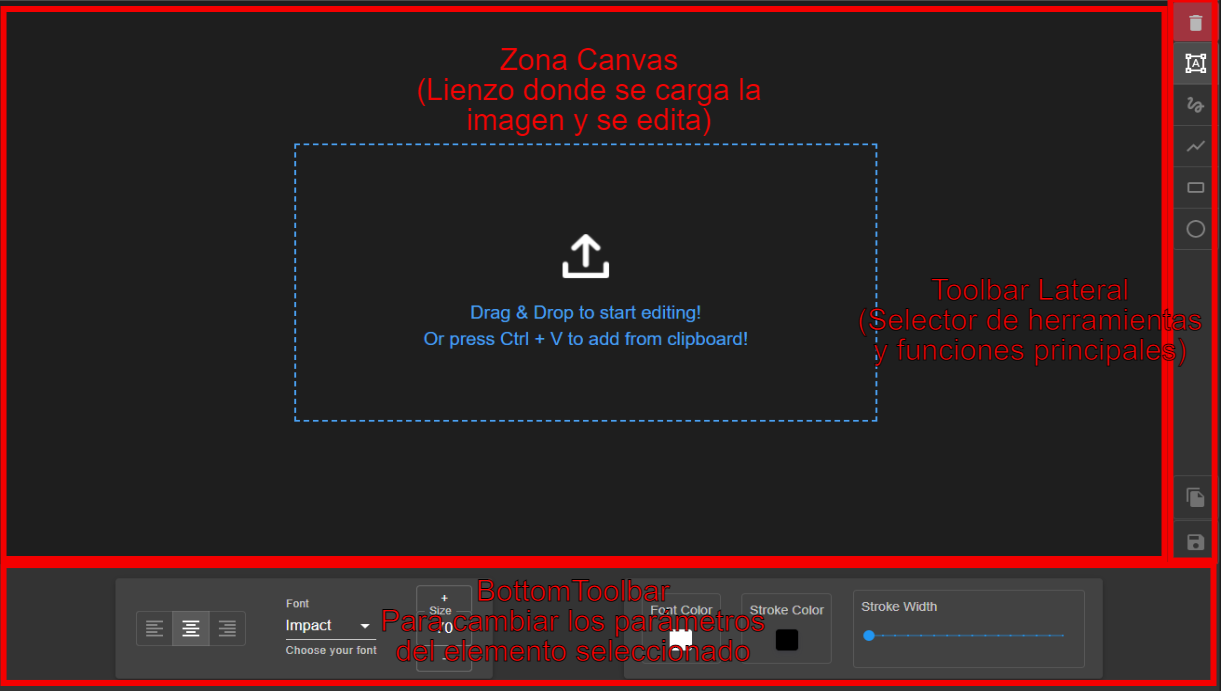
\includegraphics[scale=0.30]{img/ESQUEMA_PARTES.png}
  \caption{Esquema de las principales partes de la aplicación}
\end{figure}

\newpage
La principal ventaja que tiene dividir la aplicación en estos subcomponentes es que desde
React, podemos re-renderizar cada uno de forma individual cuando lo necesitemos, de esta forma
no hay que renderizar toda la página cada vez que se cambia un simple selector, sólo la o las
partes necesarias, lo que mejora notablemente el rendimiento y da una experiencia mucho mas
fluida al usuario.
\\\\
Tras crear una base de placeholders que diferencien las distintas partes planificadas
de la aplicación, comenzamos con el desarrollo de las primeras carácterísticas 
partiendo de las primeras historias de usuario.

%Justificar por qué esa biblioteca y hablar un poco de ella
\section{Biblioteca de canvas para React: KonvaJS}
Para empezar a elaborar la aplicación, comenzamos por la funcionalidad más básica necesaria
cargar multimedia en el lienzo del editor, necesitamos una imagen para editar y por
ende se comenzó por crear esta funcionalidad.
\\
Ya se había elaborado una carga de imagen en las demos de la fase de planificación, 
puramente en html y javascript, empleando el elemento HTML Canvas, en estas demos 
se pudo comprobar que para la tarea que queríamos realizar manejar el elemento
canvas desde el DOM\cite{DOM} no era eficiente, ni aprovechaba todas las ventajas 
de React.
El elemento HTML canvas es un mero array de píxeles, no hay manera de diferenciar 
los objetos dibujados en el canvas una vez dibujados, son solo píxeles de otro color,
para hacer esto, tenemos que tener los objetos almacenados en memoria y actualizar el
canvas repintando todos los objetos cada vez que se modifica algo, esto no es una 
tarea fácil, ya que hay que gestionar entre otras cosas la frecuencia de actualización
del canvas (frames per second) y asegurarse de que el código es eficiente, ya que 
no es una tarea trivial en potencia de procesado necesaria.
Por ende y tras investigar las distintas posibilidades se decidió utilizar una 
biblioteca específica para gestionar el elemento canvas HTML para React, de este
modo, podemos aprovechar las carácterísticas de React y olvidarnos de gestionar 
la frecuencia de actualización del canvas, ya que la biblioteca lo repinta cada vez
que se hace un cambio, además de tener una forma unificada de instanciar los objetos
que estan pintados en el canvas, todos los objetos que se pintan son instancias de 
hijos de clases propias de la biblioteca o directamente son instancias de clase de la 
misma.
\\\\
Tras investigar y barajar varias opciones se terminó decidiendo elegir KonvaJS 
\cite{KonvaJS} como biblioteca, primero porque era específica de React
(aunque tiene versiones para Vue.js ) 
y segundo, porque contaba con clases y métodos bastante interesantes para una aplicación
como un editor, el resto de bibliotecas estaban mucho mas enfocadas a animaciones, sin 
embargo, KonvaJS permite mucha mas inteacción con el lienzo, que es lo principal en un
editor.
%Como funciona
\section{El Drag\&Drop principal}
%Lo primero que se empezó a hacer despues de poder añadir la imagen
Habiendo importado las dependencias necesarias para KonvaJS\cite{KonvaJS} en el proyecto,
se comenzó a implementar la funcionalidad mas básica y necesaria del editor, para editar,
necesitamos tener algo que editar. 
\\
En este punto había que tener en cuenta una de las principales intenciones del proyecto,
se debía poder utilizar el editor sin necesidad de descargar nada o utilizar archivos
guardados en la memoria local, es decir, que había que poder añadir contenido desde 
el portapapeles al editor, aunque también se da la opción de usar contenido local.
\\
Para comenzar, se creó un componente de React que se renderizaría cuando no haya 
nada cargado en el lienzo.

\begin{lstlisting}[caption={Renderizado condicional del componente del DragandDrop}]
  {//If there is no image, show draganddrop input
  ( this.state.image == null ) ?
      <DragandDrop imgLoader={this.imageLoader.bind(this)}/> 
      : 
      <SecondaryDragandDrop 
          imgLoader={this.createNewSecondaryImage.bind(this)}
      />
  }
\end{lstlisting}

Este componente consiste en un área de drop donde el usuario puede añadir el archivo 
haciendo drag desde su PC, se emplea el evento OnDrop para leer el fichero, si es
del formato correcto, se lee y se manda al componente padre (editor) para cargarlo en 
el canvas.
\\
El canvas se carga haciendo uso de la biblioteca KonvaJS \cite{KonvaJS}, desde React 
no tenemos un elemento canvas, tenemos el componente Stage de la biblioteca, así que 
lo cargamos en él, haciendo uso de los métodos de la biblioteca.
\\\\
El canvas se renderiza desde el principio de la aplicación, al principio se pensó 
en hacer un renderizado condicional al igual que con la zona de drop, pero el Stage
(el canvas en el DOM), es el elemento más importante de toda la aplicación
que además es necesario para el funcionamiento base de la propia aplicación 
(no se puede editar nada sin él, es el propio lienzo), así que no tenía mucho sentido
condicionar su renderizado ya que no aportaba nada,
para evitar posibles complicaciones simplemente se renderiza en oculto con ancho y alto
de 0.
\\\\
Cuando se carga una nueva imagen necesitamos calcular qué tamaño tendrá el lienzo, 
cada imagen puede tener un tamaño completamente diferente y queremos que la aplicación
tenga consistencia, es decir, que el usuario sienta que siempre tiene un área de edición
parecida independientemente de la resolución de la imagen.
Para ello debemos tener dos cosas en cuenta, el tamaño de la zona de edición del usuario,
que depende de su propia pantalla y el tamaño original de la imagen.
La correlación de la imagen siempre habrá que mantenerla para que no se deforme la 
imagen base, la calculamos y manteniendo esa correlación ajustamos la imagen al tamaño
disponible dejando algo de espacio por estética (para las imágenes demasiado pequeñas, 
no se efectua ajuste porque no es necesario).

\begin{lstlisting}[caption={Método para calcular el tamaño del lienzo a partir de una imagen}]
  calculate_resize(correlation, width, height){
        let pixel_margin = 100
        //wide photo
        if( correlation <= 1 ){
            //image too small, dont correct
            width = (width > 400 ? width - pixel_margin : width)
            //
            if( correlation * width < height ){
                height = (correlation * width) - pixel_margin
                width = width - pixel_margin
            } else {
                width = height * (1/correlation) - pixel_margin
                height = height - pixel_margin
            }

        //long photo
        } else {
            //image too small
            height = (height > 400 ? height - pixel_margin : height)
            //
            if( height * (1/correlation) < width ){
                width = height * (1/correlation)
                //height = height
            } else {
                width = width - pixel_margin
                height = correlation * width - pixel_margin
            }
        }

        return {
            width: width,
            height: height
        }
    }
\end{lstlisting}

\newpage
\section{La primera herramienta: Añadir Texto}
Ya que tenemos el mínimo necesario, que es tener una imagen que empezar a modificar, 
comenzamos a implementar la primera funcionalidad, al ser un editor especialmente
enfocado en facilitar la edición de memes, se comenzó por la funcionalidad mas básica
para hacer un meme, añadir texto encima de una imagen base.
\\\\
Como hemos comentado, desde React tenemos una abstración del canvas html llamada Stage,
dentro de este, podemos añadir cualquier objeto nodo de la biblioteca KonvaJS y el texto
ya existe como una clase. Para comenzar el desarrollo añadimos un texto temporalmente
desde el render al que se fue dotando de funcionalidad.
\\
Además del texto, la biblioteca cuenta con otra clase llamada transformer, que sirve 
para mostrar una caja de transformación alrededor de cualquier otro nodo. El problema
de esta clase es que el comportamiento del transformer por defecto consiste en 
reescalar el nodo, en un texto lo que queremos es que las letras se distribuyan
equitativamente por todo el espacio ya que el tamaño se define a parte.
\\\\
Para ello, se ha sobrecargado el comportamiento del evento de transformación del texto.
Ya que sobrecargamos una funcionalidad básica de la clase propia de la biblioteca, se 
decidió crear una clase propia partiendo de la base de la biblioteca, la clase CvText
que encapsula el renderizado del nodo base de Konva con nuestras funcionalidades personalizadas.
Realmente no es una clase, es un componente funcional de React, es decir, es una 
función que devuelve un render, en las nuevas versiones de React se recomienda usar
componentes funcionales ya que simplifican el código y practicamente tienen las mismas
capacidades que las clases gracias a los React-Hooks \cite{React-Hooks}, siempre que 
no se ha necesitado instanciar un componente para llamar métodos asociados a él 
(esta es la principal diferencia, al ser una función no tiene métodos propios) se han
creado componentes funcionales como marcan las buenas prácticas actuales del lenguaje.
\\\\
Por defecto, los métodos cuentan con un tamaño (ancho y alto) y una propiedad de escalado
en X y en Y, el transformador cambia la escala, por ende cada vez que el nodo se transforma
reseteamos la escala y la aplicamos al tamaño real del nodo. 

\newpage

\begin{lstlisting}[caption={Sobrecarga del reescalado del nodo CvText}]
const scaleReset = () => {
    let text = textRef.current

    text.setAttrs({
        width: text.width() * text.scaleX(),
        scaleX: 1,
        height: text.height() * text.scaleY(),
        scaleY: 1
    })
}
\end{lstlisting}

Para mover el nodo por el lienzo contamos con la propiedad drag de la biblioteca, al ser
una funcionalidad tan básica, venía también preimplementada en la biblioteca.
Mas adelante veremos que esta propiedad se hace condicional ya que no siempre queremos
poder mover cada nodo al clickar encima pero en este punto se añadió directamente para
simular el comportamiento que queríamos que tuviese el nodo.
\\\\
Ahora viene la funcionalidad mas importante del texto, poder editar los 
carácteres, para ello, hemos hecho uso del elemento HTML textarea, es mucho mas
fácil que crear todo un sistema de edición dentro del lienzo, ya que como hemos comentado
no es más que un array de píxeles. Pero, queremos que el usuario lo perciba como si estuviera
realmente editando el texto de dentro del lienzo de una forma dinámica,
hay un evidente problema con esto ya que la textarea HTML por defecto es una caja opaca
sin estilo alguno, para solucionar este problema se ha creado un método dentro del 
componente CvText que lee el estilo del texto dentro del lienzo y calcula una serie
de reglas CSS que se definen a partir del texto base (el texto de Konva \cite{KonvaJS})
y se aplican a la textarea HTML.

\begin{figure}[!h]
  \centering
    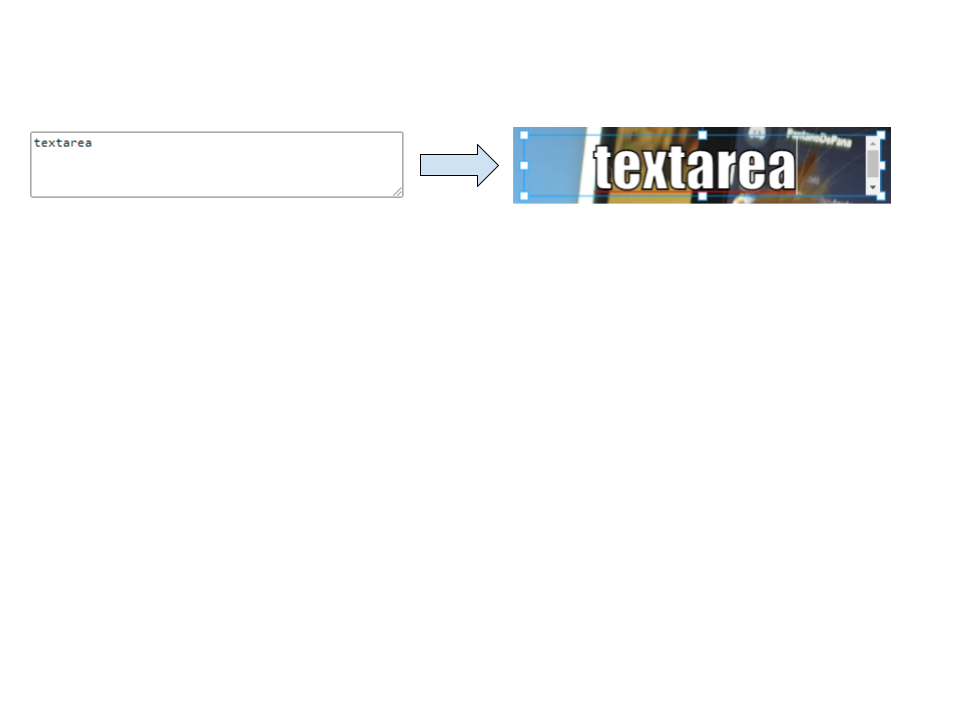
\includegraphics[scale=0.55]{img/textareadiff.png}
  \caption{Ejemplo de cambio de estilo de la textarea por defecto y el aspecto tras las reglas css calculadas a partir del texto del canvas}
\end{figure}

%\newpage
La textarea se genera encima del texto del lienzo y se oculta el texto del canvas,
de este modo, el usuario tiene la sensación deseada aunque realmente no está tocando
el lienzo, cuando el area textpierde el focus desaparece y se vuelve a renderizar el 
texto en el lienzo con el valor actualizado.

No todos los navegadores tienen exactamente el mismo comportamiento así que hubo que 
introducir algunas reglas extra o excepciones dependiendo del navegador. 
\\\\

\section{El lienzo: Stage}

Ahora que tenemos el primer nodo básico con el funcionamiento deseado, necesitamos que
el usuario sea capaz de añadir y eliminar textos, para ello debemos almacenar los 
nodos que se muestran en el lienzo y repintarlos cada vez que haya algún cambio.
\\\\
Para ello creamos un array que almacena los nodos en el estado del componente, al ser 
un array, React no detecta los cambios automáticamente, así que debemos lanzar manualmente
el repintado del lienzo cuando sea necesario, de este modo tenemos mas control sobre 
el renderizado y el rendimiento.
\\\\
Mas avanzado el desarrollo, nos encontramos con un problema en este punto. En el desarrollo
de React, se emplea JSX\cite{JSX}, que es una capa de abstracción sobre los métodos de React 
para hacer mas intuitivo el desarrollo usando la sintasis de un lenguaje de marcado,
en este caso HTML.
\\\\
Por esto, lo que contiene el array de items no son realmente objetos que se re-renderizan
sino una función propia de React que instancia un objeto camuflado en forma de HTML (JSX\cite{JSX}).
Esto hace que no podamos cambiar las propiedades de los nodos ya renderizados, ya que
en las siguientes iteraciones del render, React detecta que ese nodo ya está instanciado,
el render no hace nada y los cambios no se aplican. 
\\\\
Para solucionar esto hicimos uso de la función React.cloneElement al re-renderizar
un objeto diferente pero que es un clon del anterior (con propiedades modificadas)
que ya está instanciado en caché el re-render sustituye la instancia por la del clon,
con los parámetros cambiados y pero manteniendo los demás que no han sido modificados.

\begin{lstlisting}[caption={Render del array de nodos}]
{ //Renders all items into the canvas
  this.state.itemArray.map(Item => (
      React.cloneElement(
          Item,
          { draggable: (this.state.selectedTool == "SelectorAndText") }
      )
  ))
}
\end{lstlisting}

De este modo los nodos solo pueden ser arrastrados cuando la herramienta correcta está
seleccionada, cuando cambia la herramienta se lanza un re-render del stage y se actualizan
las propiedades de los nodos.

\newpage
\subsection{Los handlers}

Ahora que tenemos una manera de almacenar y modificar los textos, 
el usuario necesita una forma de crearlos y eliminarlos, para ello necesitamos 
detectar los eventos, al igual que con el texto, también necesitamos tratar los eventos
para cada herramienta.
No todas las herramientas tienen los mismos eventos ni se comportan igual ante los eventos,
por eso la forma de capturar cada evento es con un método handler genérico que lleva a un 
switch que redirige el evento al handler correspondiente dependiendo de la herramienta seleccionada.
\\
Los eventos se capturan en el componente Layer, es un componente intermedio propio de KonvaJS\cite{KonvaJS},
que está entre el Stage y los nodos que se renderizan.

\begin{lstlisting}[caption={Enlazado de los handlers al componente layer que captura los eventos}]
<Layer
  ref={this.mainLayerRef}
  onMouseDown={this.handleCanvasMouseDown.bind(this)}
  onMouseMove={this.handleCanvasMouseMove.bind(this)}
  onMouseUp={this.handleCanvasMouseUp.bind(this)}
  onMouseLeave={this.handleCanvasMouseLeave.bind(this)}

  onDblClick={this.handleCanvasDblClick.bind(this)}
>
\end{lstlisting}

Aquí podemos ver un ejemplo de handler genérico del canvas donde se redirige al handler correspondiente

\begin{lstlisting}[caption={Sobrecarga del reescalado del nodo CvText}]
  handleCanvasMouseDown(e){
    switch(this.state.selectedTool){
        case 'SelectorAndText': 
            handleSelectorMouseDown.bind(this)(e)
        break

        case 'FreeLine':
            handleFreeLineMouseDown.bind(this)(e)
        break

        case 'StraightLine':
            handleStraightLineMouseDown.bind(this)(e)
        break

        case 'Rectangle':
            handleRectangleMouseDown.bind(this)(e)
        break

        case 'Ellipse':
            handleEllipseMouseDown.bind(this)(e)
        break
    }
}
\end{lstlisting}

En principio todo este sistema de handlers no se implementó, ya que no era necesario 
porque aún no había mas herramientas, en las metodologías ágiles vas implementando según
las funciones que vas necesitando por tanto simplemente se enlazó el handler al evento
de doble click. 
\\\\
El handler crea un nuevo componente de texto (una instancia de nuestro componente propio: CvText),
lo inserta en el array de nodos del editor y lanza un re-render para que se muestre.
Además en nuestra encapsulación del CvText cuando se crea el nodo por primera vez se
llama automáticamente al método que genera el textarea de edición ya que recién creado
el usuario, muy probablemente querrá editar su contenido.
\\
Para evitar que se lance cuando se clona el elemento, se ha hecho uso de los React Hooks\cite{React-Hooks}
propios de los componentes funcionales.
\\\\
Para el resto de herramientas todo este sistema funciona igual, se detecta un evento, se
redirige al handler de la herramienta correspondiente y se crea un nuevo elemento del tipo
deseado. Dependiendo de cada herramienta el evento con el que se crea el nodo es distinto y el 
comportamiento de los handlers cambia, pero la estructura es la misma. 
\\\\
Hay varios handlers extra que se diferencian de los handlers de las herramientas para los
eventos de teclado como ctrl + v para cargar una imagen o supr para borrar un nodo.
El funcionamiento general es el mismo pero no se necesita condicionar la herramienta seleccionada
para el borrado simplemente se ejecuta una función que obtiene el nodo seleccionado, lo
destruye de la caché, lo saca del array y re-renderiza el lienzo.
\\
Y para la carga de imágenes mediante ctrl + v, se lee el evento, se busca el fichero asociado
en el portapapeles y se envía al método de carga de imagen principal o secundaria dependiendo
de si hay una imagen base cargada.

\newpage
\section{Herramienta: Selector}
Ya que podemos crear el texto necesitamos poder cambiar entre textos, para ello, se creó
la primera herramienta, el selector, que mas adelante se fusionó con la creación de texto
por puro pragmatismo, había que estar cambiando de herramienta innecesariamente después
de crear un texto, por eso se decidió unir ambas funcionalidades en una sola herramienta,
para el resto de herramientas no podía ser así ya que coincidian los eventos, el click 
de selección, con por ejemplo, el click que comienza la creación de una línea.
\\\\
La herramienta selectora se encarga de activar y mostrar el componente Transformer en
el nodo que desea el usuario.
Para ello, teníamos que poder diferenciar los nodos del canvas, KonvaJS\cite{KonvaJS}
nos permite encontrar el nodo sobre el que se ha hecho click a partir del evento, 
aprovechando esto, simplemente tomamos el nodo clickado y lo introducimos en el componente
transformer, excepto si lo que se clicka es la imagen base, en cuyo caso vacíamos el transformer
para deseleccionar cualquier nodo.

\section{Cambio de propiedades: BottomToolbar}

%Como funciona el componente bottomtoolbar y como va cambiando
%Comentar aquí todo el tema handlers, updates etc y como se sincroniza
%con el cambio de item, es igual para todas las herramientas

Además de cambiar el texto, el usuario debe poder personalizar los elementos que añada al lienzo,
para ello y como teníamos planeado, se añadió una barra de herramientas que irá cambiando
dependiendo del nodo que esté seleccionado.
\\\\
En este punto del desarrollo solo se podían añadir texto, así que se comenzó creando un componente
BottomToolbar para cambiar las propiedades del texto.
Para ello, en primer lugar necesitamos controladores con los cuales el usuario pueda cambiar 
esas propiedades de forma sencilla, para ello hicimos uso de Material-UI\cite{materialui}, una 
biblioteca de componentes de React con estilo de material design.
\\
\begin{figure}[!h]
  \centering
  \noindent\makebox[\textwidth]{
    
\includegraphics[scale=0.3]{img/bottomtoolbar.png}}
  \caption{Aspecto de la BottomToolbar de edición de texto}
\end{figure}

Todos los componentes usados pertenecen a la biblioteca por defecto de Material-UI excepto el
selector de color, que es un proyecto open source independiente hecho a partir y para Material-UI
llamado material-ui-color\cite{material-ui-color}.

\newpage


\begin{figure}[!h]
  \centering
  \noindent\makebox[\textwidth]{
    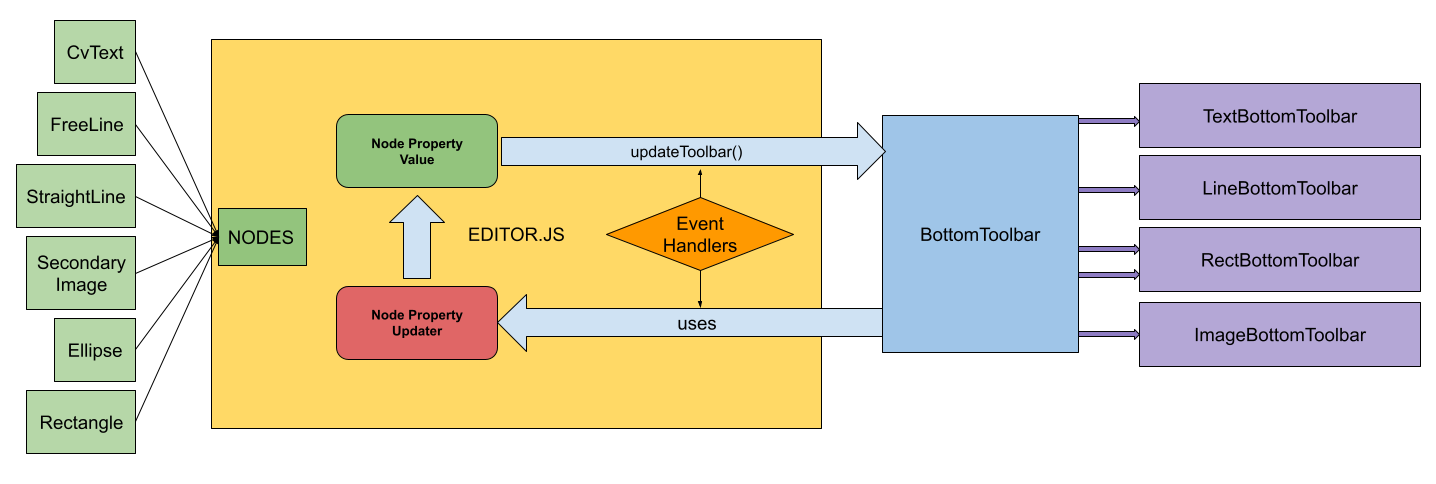
\includegraphics[scale=0.45]{img/FlujoDatosBottomToolbar.png}}
  \caption{Esquema del flujo de datos entre los nodos del lienzo y la BottomToolbar}
\end{figure}





\section{Cambio entre herramientas: Toolbar}



\section{Herramienta: Lineas}
  \subsection{Herramienta Freeline}
  \subsection{Herramienta StraghtLine}
\section{Herramienta: Formas Geométricas}
  \subsection{Herramienta: Rectángulos}
  \subsection{Herramienta: Elipses}
\section{Herramienta: Imágenes superpuestas}
Como no podía faltar en un editor de memes

%konva

\iffalse
Esquema para luego redactar bien:
- A partir de la demo rehice todo para adaptarlo a la libería 

- Lo primero fue hacer que se pudiera añadir una foto base (DragAndDrop y Konva canvas)

- Explicar todo tema lienzo, cálculos etc..

- Se añadió poder quitar la foto y volver a añadir otra

- Comenzamos el poder añadir texto

- todo tema texto, textarea, propiedades, drag, transformador, lo de adaptar el texto al tamaño 
de la caja bla bla 

- Comienzo de la toolbar para poder poner el texto bonito

- Tema toolbar, material-ui, como mandamos la info desde la toolbar al texto y lo actualizamos
 bla bla

- Hablar de ajustes varios, tema eventos etc.. clicks handlers bla bla

- Añadido el ctrl + v de imagen principal (esto quizá explicarlo después para juntar todo el 
tema texto)

- Handleo de varios textos diferentes

- Cuando ya se cambiaban los textos desde la toolbar ahora como se cambia la toolbar 
para que coincida con las opciones del texto

- Hablar un poco de tema componentes funcionales vs clases (todos los cambios que se hicieron)

- PRIMERA TANDA DE TESTS (preguntar a JJ si explicar esto todo luego o aquí)

- Además de texto ahora a añadir mas cosas, Imágenes y sus transformaciones

- Hablar del tema lineas, como se movian las cosas al pintar encima, la lógica de las herramientas
  como se ha solucionado, porque se ha hecho así y el React.clone()

- [pensar lo que falta por aqui]

- tema eventos, copiar pegar, guardar etc

-production build

-despliegue

\fi

\newpage
\section{Tests}

Como es costumbre en las metodologías ágiles, se ha testeado, en la medida de lo posible,
todo el código que se ha ido desarrollando según se iba añadiendo a la aplicación.
Para ello necesitabamos escoger de que manera íbamos a testear nuestro código, se barajaron
varias opciones, como el módulo de tests-utils que trae react-dom \cite{react-dom} o jest, 
pero estos módulos no encajan lo suficientemente bien con una aplicación como un editor, 
algo que es muy interactivo y gráfico requería testearlo también de forma gráfica. Por ende
se terminó escogiendo Cypress \cite{cypress} que es una herramienta que simula un navegador de
forma gráfica y genera los eventos, además cuenta con un módulo para React \cite{cypressReact} que permite montar
y testear componentes individualmente, además de comprobar el estado (state) de React, cosa
que no permiten la mayoría de aplicaciones de testeo gráfico, ya que, en el navegador los
componentes no existen como tal, sólo el código HTML que genera React a partir de estos.

\begin{figure}[!h]
  \centering
  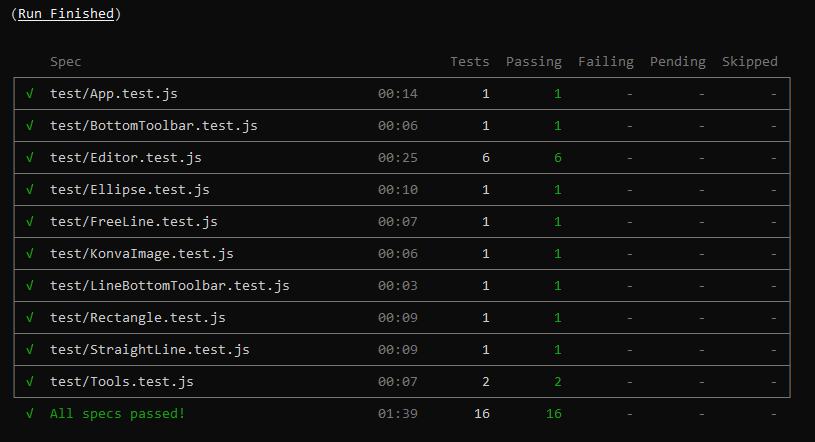
\includegraphics[scale=0.6]{img/TestsOK.png}
  \caption{Resultado de la ejecución de los tests de cypress, run-ct}
\end{figure}

Lo ideal es testear el 100\% del código de la aplicación, aunque en la realidad llegar a esto
es bastante complicado, se ha intentado cubrir la mayor parte posible, para ello se han creado
tests para cada historia de usuario que hemos definido, crear el test era requisito para considerar
terminada la historia de usuario y como es lógico el test debía testear la funcionalidad que 
proponía la HU. Hubo una excepción en las primeras historias de usuario que se completaron
no se testearon directamente, ya que el testeo se comenzó algo mas tarde para esperar a 
que la aplicación tuviera ciertas funcionalidades básicas completas ya que en el inicio es
muy fácil que ciertas partes cambien drásticamente y así evitar rehacer tests de forma innecesaria,
de todos modos, estas partes fueron testeadas en cuando se empezaron a desarrollar los tests.

\newpage
\section{Despliegue de la aplicación}

Ahora solo nos falta desplegar la aplicación, en nuestro caso se va a desplegar esta primera 
versión utilizando el servicio de Github Pages \cite{GithubPages}.
\\
Como comentamos al inicio, para crear esta aplicación empleamos el paquete create-react-app \cite{create-react-app},
este paquete cuenta con scripts que ayudan en el despliegue de la aplicación y crean una 
versión optimizada del código.
Como era uno de los objetivos del desarrollo, la aplicación ha sido desarrollada pensando
en hacer que, aunque sea una aplicación multimedia, no se requiera de un servidor potente que
soporte mucha carga, es decir, es puro front-end, así que sólo necesitamos que el servidor
envíe código HTML, CSS y los scripts de Javascript, no tiene que procesar nada relativo a las
ediciones que haga el usuario ya que esas operaciones se efectuan en el cliente.
\\
Esto nos permite emplear hostings ligeros para el despligue, 
%en nuestro caso hemos decidido
%emplear Github Pages por 3 razones, el proyecto ya estaba siendo desarrollado en Github,
%el paquete create-react-app \cite{create-react-app} tiene soporte para Github Pages \cite{GithubPages}
%y por qué no decirlo, es gratuito y funciona bastante bien.
los hostings mas usados son Azure, Firebase o AWS aunque son bastante flexibles son hostings 
bastante potentes y de pago, gracias a como está construida la aplicación no necesitamos tanto,
así que vamos a emplear Github Pages por varias razones, el paquete 
create-react-app \cite{create-react-app} tiene soporte para Github Pages \cite{GithubPages}
y por qué no decirlo, es gratuito y funciona bastante bien.
\\
Para el despliegue se han seguido las instrucciones que nos da la documentación de 
create-react-app para hacer deploy en Github Pages \cite{GithubPagesDeploy}.
Es bastante simple, añadimos la configuración de la ruta donde se hará el deploy e instalamos
el paquete npm gh-pages \cite{gh-pages}, que es el que recomienda la documentación oficial.
Y añadimos unos scripts que hacen uso del paquete para el deploy, al ejecutar el script
crea una branch que sirve como source estático de la web.
\\\\
El despliegue puede probarse en el siguiente enlace: \url{https://bytevictor.github.io/memeHub/}

	% Presupuesto

	% Conclusiones
	\chapter{Conclusiones y trabajos futuros}

%Si estoy satisfecho

%Has conseguido cumplir los objetivos

%se ha seguido la planificacion

La realización de este trabajo me ha permitido adquirir una gran cantidad de conocimiento
en tecnologías actuales de desarrollo web como son React y Javascript, además he podido
poner en práctica mucho de lo aprendido en la carrera, tanto de programación como de 
planificación u optimización.
\\\\
Ha sido un primer verdadero proyecto como ingeniero cuyo resultado ha sido 
un producto funcional y útil.
Este editor ha cumplido el objetivo que se propuso, posibilitar la edición de imágenes
sin necesidad de descargar nada en ningún momento, es un editor fluido y que cuenta 
con las funciones básicas necesarias para poder editar imágeness.
\\\\
Estoy satisfecho con el trabajo realizado y quiero seguir avanzando este proyecto hasta 
convertirlo en un editor completo y competitivo, quiero añadir muchas mas funcionalidades
tanto dentro del editor, con nuevas herramientas y funciones (recorte de imágenes, 
multiselección de nodos, etc.) como fuera del editor. 
Me gustaría crear una web de imágenes
que gire entorno al editor, donde los usuarios puedan registrarse y guardar los resultados
de su edición además de poder repostear el contenido en las principales redes sociales
de forma simple.
\\\\
Además creo que este proyecto será una buena carta de presentación de cara al mundo
laboral para trabajar en el área de desarrollo web, área en la que estoy especialmente
interesado.

	% Trabajos futuros


	
	\newpage
	\bibliography{bibliografia}
	\bibliographystyle{plain}
	
\end{document}

